\subsection{Taxonomy Details}
\label{app:taxonomy}

\subsubsection{Taxonomy Definition}
\label{app:taxonomy-definition}

\noindent \textbf{Scope.}
ALE evaluates whether generalist computer-use agents, operating through digital interfaces, software
tools, files, and APIs, can complete valuable professional work across fields. The taxonomy centers
on workflows whose primary outputs can be produced at a computer, depend on domain expertise,
and yield artifacts that are objectively evaluable.

\noindent \textbf{Occupational backbone.}
We use SOC 2018 as the occupational backbone and O*NET to interpret occupational content through
linked task, work-activity, and tools-and-technology records~\citep{bls2018soc,peterson2001onet,onet302database}.
SOC 2018 provides a standard classification of U.S. occupations, while O*NET provides
occupation-level records describing work content, activities, tasks, and technology use. SOC 2018
describes the structure of U.S. work across 23 major groups, 98 minor groups, 459 broad occupations,
and 867 detailed occupations. To derive ALE's workflow-level taxonomy, we screen these occupation
records for in-scope digital workflows, consolidate the retained occupational evidence into
subdomains, and supplement SOC/O*NET where stable frontier workflows are absent or under-specified.

\noindent \textbf{Screening procedure.}
The initial screen applies the scope definition to the 1{,}016 entries in O*NET 30.2 Occupation
Data~\citep{onet302database} using a fixed GPT-4o mini prompt at temperature~0. Each prompt
instance includes the SOC code and title, O*NET description, task statements, work activities, and
technology examples. After O*NET variants are consolidated under shared SOC base codes, 117 unique
SOC base codes remain.

\noindent \textbf{Subdomain construction.}
The screening stage identifies occupation-level evidence, which we then organize into workflow-level
subdomains. We group SOC codes whose task statements, work activities, and tools-and-technology
records describe a common class of artifact-producing professional work. Field, methodology, and
work product are the primary dimensions used to set subdomain boundaries, with LLM-assisted
research and domain-expert review used to check borderline assignments. A SOC code can be assigned
to more than one subdomain when its work content contains separable workflows. This process yields
51 SOC-anchored subdomains.

\noindent \textbf{Frontier extension.}
SOC/O*NET anchors the taxonomy in established occupations. ALE further adds a frontier supplement
for emerging digital workflows not yet represented in SOC 2018 but already present in current
research and professional practice, as reflected in recent NIH, NSF, and field-specific technical
roadmaps~\citep{nih2021strategicplan,nsb2024sei,uschips2022,nsfchips2024,nist2023airmf}.
The supplement adds four frontier subdomains and seven extensions to SOC-anchored subdomains,
yielding \taskcount{} subdomains in total.

\noindent \textbf{Result.}
The final taxonomy contains \taskcount{} workflow-level subdomains grouped into \clustercount{}
domains.

\subsubsection{Industry Landscape Review}
\label{app:industry-landscape}

\noindent \textbf{Collection context.}
Subdomain workflow landscapes provide collection context for task workflows within each subdomain.
Each landscape summarizes the work setting, practitioner roles, digital inputs, workflow
dependencies, and output artifacts associated with a class of professional workflows. The records
are based on field references, workflow documentation, LLM-assisted research, and expert
review. They are used to organize candidate task families and to check that collected tasks specify
realistic inputs, practice-appropriate deliverables, and verifiable success criteria. This section
includes four illustrative subdomain workflow landscapes.

\subsubsection{Manufacturing \& Industrial Operations}
Manufacturing \& Industrial Operations covers workflows that turn CAD geometry, bills of materials,
process specifications, and production targets into routings, toolpaths, line layouts, control logic,
and inspection plans. A recurring handoff risk is consistency between the digital plan and the physical
process: controller dialects, fixture geometry, alarm priorities, and tolerance stacks are tracked
across CAM, controls, industrial engineering, and quality review.

Work starts from a part model, material requirements, and a production target. Process planners
assign machine classes and routings; CAM programmers generate toolpaths, post G-code, and verify
cutter motion in stock simulation; industrial engineers balance station times against takt; controls
engineers write PLC logic, SCADA screens, alarm priorities, and safety interlocks; quality engineers
author SPC plans, control limits, and first-article inspection procedures. The resulting artifacts
include routing plans, posted code, simulation outputs, control files, SPC plans, and inspection
packages. When a feature drifts out of specification, the inspection record can be compared with the
process history and, when needed, route the workflow back to fixture, parameter, or toolpath
revision.

\subsubsection{Biomolecular Structure \& Design}
Biomolecular Structure \& Design covers computational workflows that precede wet-lab execution.
Typical inputs include a target hypothesis, candidate sequences or ligands, structural templates,
assay constraints, and host-organism requirements. A recurring handoff risk is consistency between the
model and the biological material: protonation states, retained waters, MSA depth, codon usage, and
assembly-junction fidelity are tracked from computational design through experimental handoff.

Work starts from a protein to inhibit, a binder to design, or a pathway to express. Computational
chemists dock candidate ligands and run molecular dynamics; structural biologists query structure
predictors for relevant conformations; protein designers filter sequences through inverse-folding
and stability models; bioinformaticians build MSAs and codon-optimize for the host; synthetic
biologists draft plasmid maps and assembly junctions. The resulting artifacts include ranked ligand
poses, structure models, sequence designs, codon-optimized constructs, plasmid maps, and design
registry entries. If a binder fails to bind, a predicted pose is contradicted, or a pathway misses
titer, the recorded assumptions may help identify the in-silico layer to revisit.

\subsubsection{3D, Animation \& Interactive Media}
3D, Animation \& Interactive Media covers workflows that convert scripts, storyboards, look briefs,
and gameplay requirements into rendered frames or runtime states. Assets move through geometry,
rigging, material, animation, lighting, compositing, and engine stages. A recurring handoff risk is
that scale, coordinate frames, import settings, color spaces, and timing metadata are preserved as
authored assets move across tools.

Work starts from a script, storyboard, and look brief. Concept artists establish the visual language;
modelers build geometry within scale, topology, and polygon-budget constraints; look-development
artists author materials and textures; riggers wire skeletons and deformers; animators key motion
against the rig and camera; lighting technical directors stage scenes; FX artists simulate particles,
fluids, and destruction; compositors layer rendered elements, while runtime engineers and technical
artists integrate assets into gameplay logic, shaders, naming conventions, and pipeline layouts. The
resulting artifacts include models, rigs, texture sets, material graphs, animation clips, lighting
setups, compositing files, and engine scenes. When a shot or build returns with incorrect scale,
color, or timing, the asset graph can help locate the layer that introduced the drift.

\subsubsection{Robotics \& Autonomous Systems}
Robotics \& Autonomous Systems covers workflows that translate task specifications and environment
models into robot descriptions, perception calibration, controllers, planners, safety logic, and
simulation assets. A recurring handoff risk is the sim-to-real gap: kinematic descriptions, sensor
transforms, controller gains, planner parameters, and simulator assumptions are tracked from digital
twin to hardware.

Work starts from a task specification, such as picking a part, reaching a target site, or navigating
a constrained route. Mechanical engineers fix the URDF and joint limits; perception engineers
calibrate sensors, validate transforms, and test perception against expected noise; controls
engineers tune gains and design safety controllers; motion planners and trajectory optimizers compose
plans under kinematic and dynamic constraints; behavior engineers connect state machines, behavior
trees, or learned policies to failure modes; simulation engineers maintain the digital twin; safety
engineers map the system to hazard analyses. The resulting artifacts include URDFs, calibration
files, controller parameters, planner configurations, behavior specifications, simulation scenarios,
and hardware-in-the-loop test records. When hardware behavior diverges from simulation, the recorded
mismatch may inform updates to the simulator, controller, or policy before the system returns to the
validation bench.

\begin{figure}[t]
    \centering
    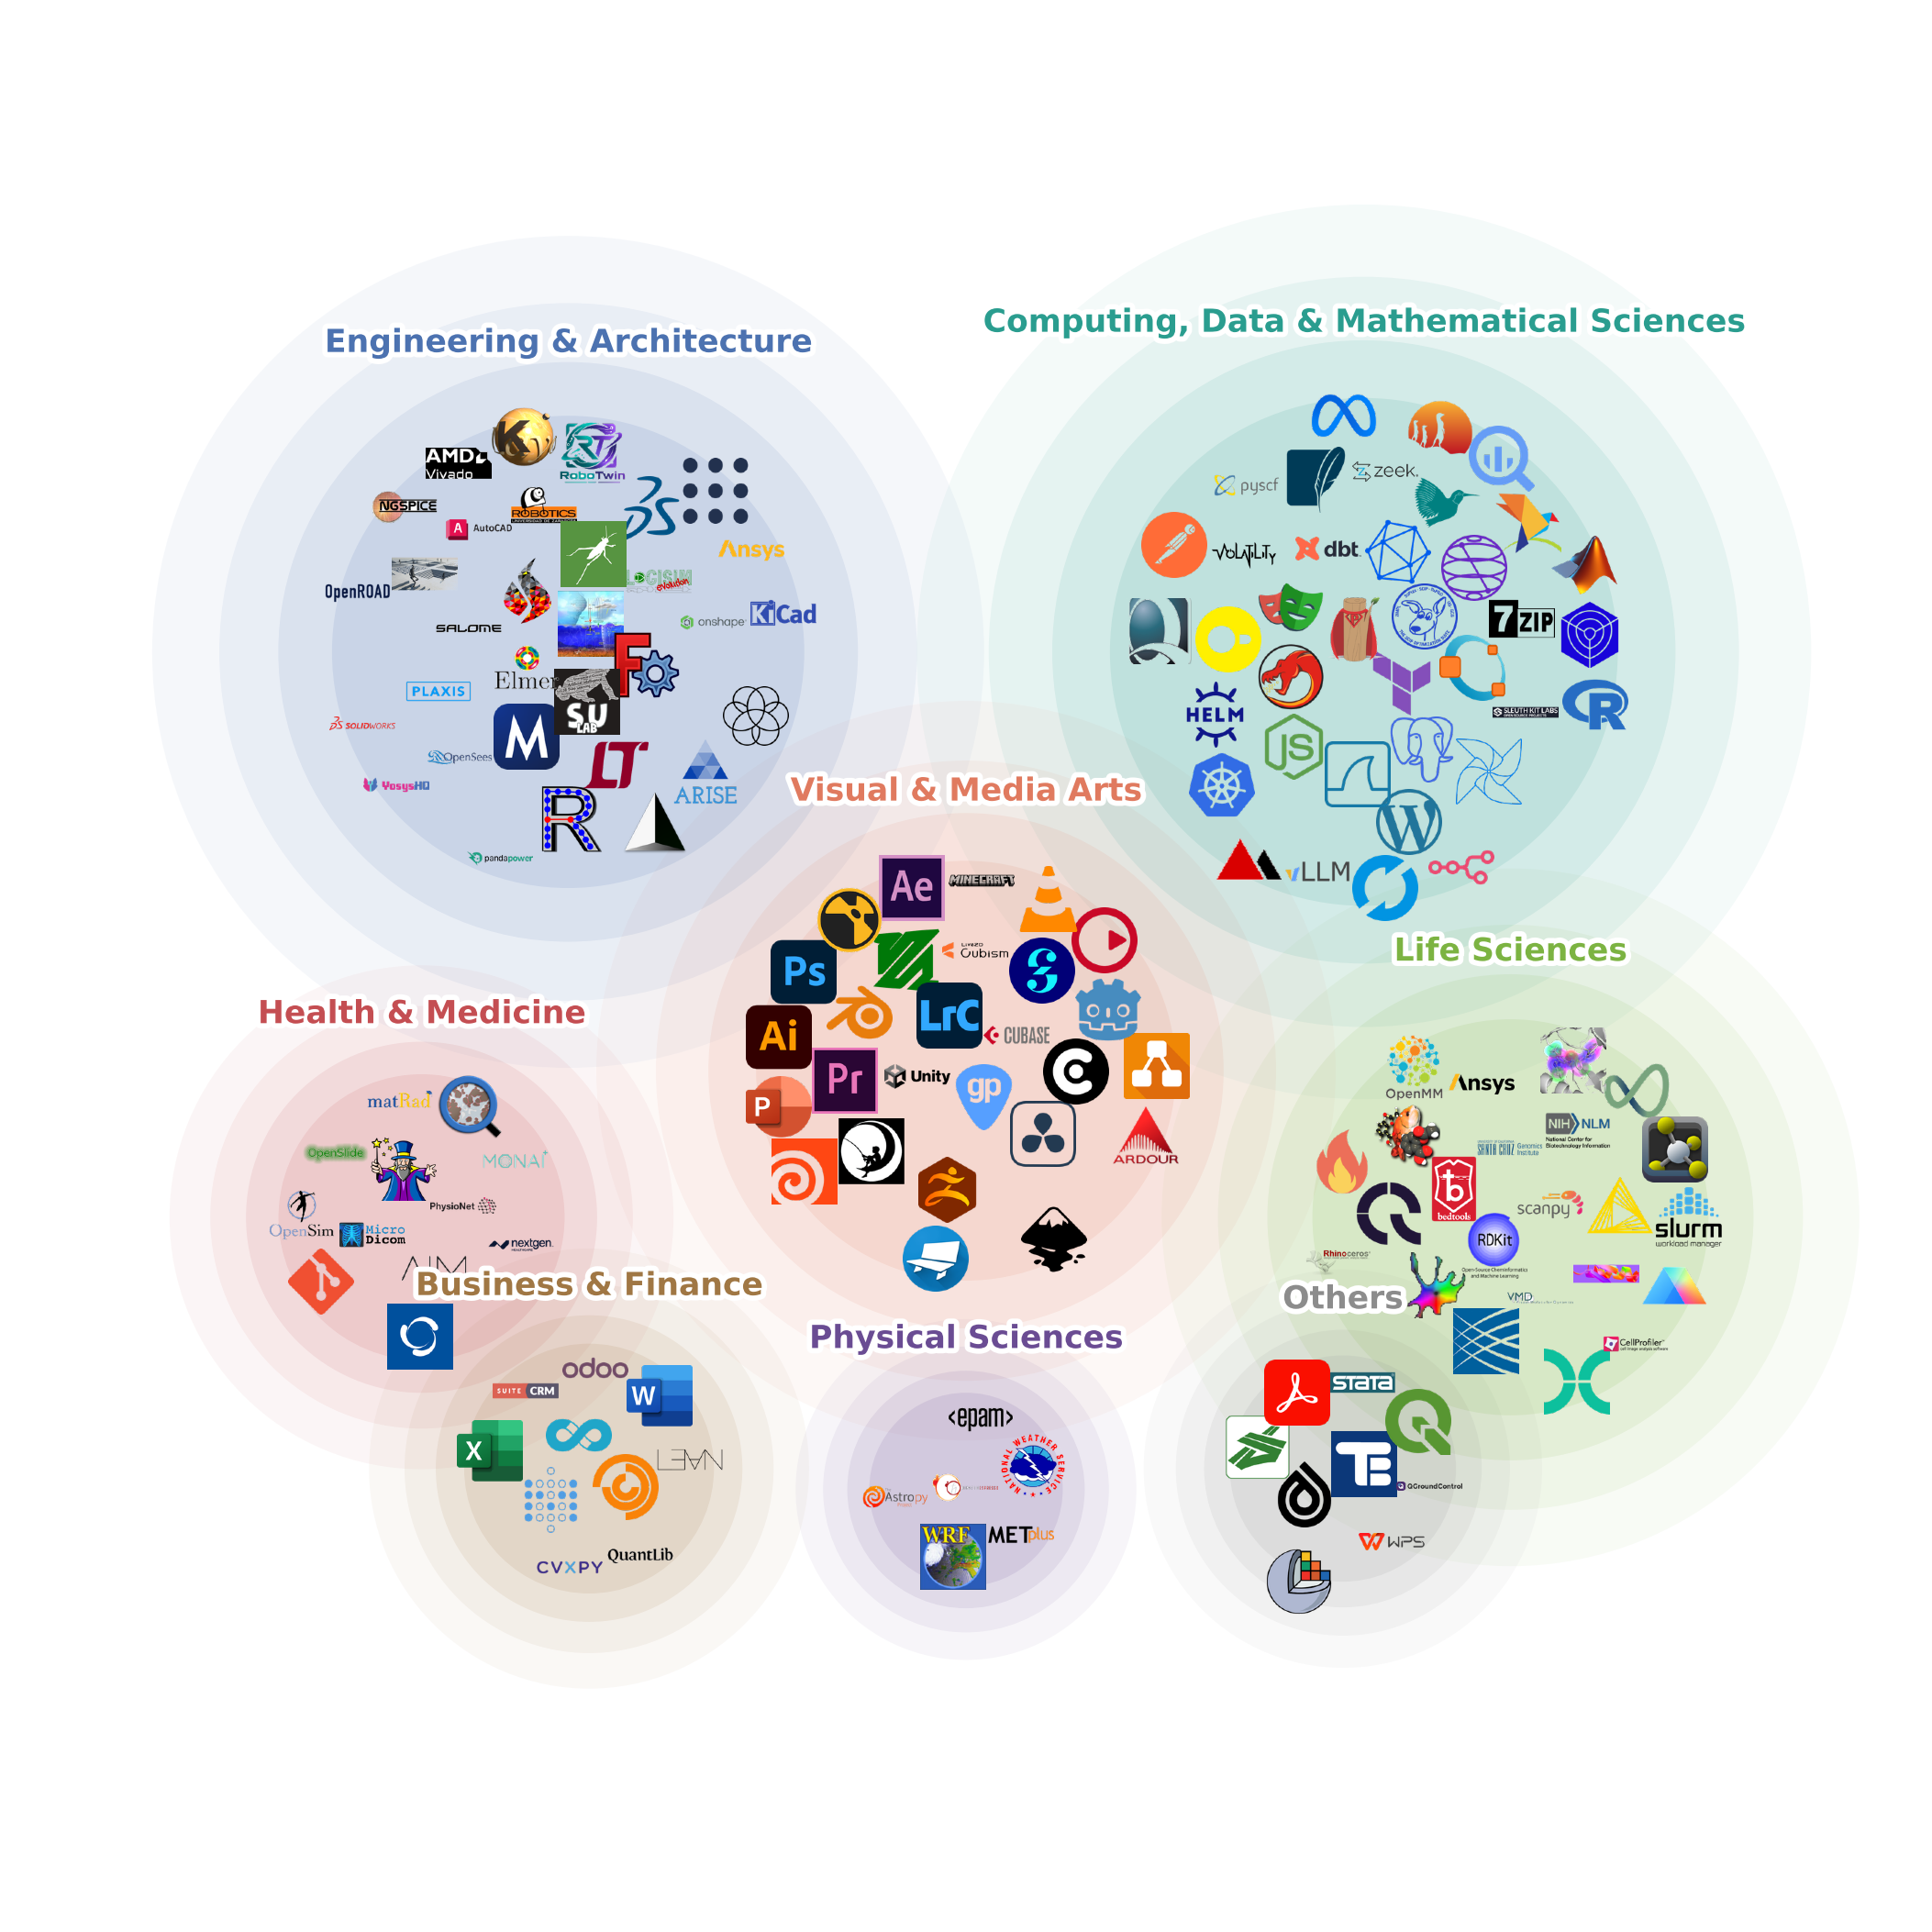
\includegraphics[width=\linewidth]{figures/build_distribution/panel_b/panel_b_constellation_by_taxonomy.png}
    \caption{\textbf{Software ecosystem covered by ALE tasks.} Each icon is a distinct application or toolchain that appears in at least one task workflow, positioned within its primary ALE domain. Overlap regions hold tools that span multiple domains (e.g., creative-suite applications shared between Visual~\&~Media~Arts and Engineering). The figure is qualitative; quantitative per-subdomain instance counts appear in Figure~\ref{fig:subdomain-distribution}.}
    \label{fig:tool-constellation}
\end{figure}
